\RequirePackage[l2tabu, orthodox]{nag}
%
    % http://www.tug.org/texlive/Contents/live/texmf-dist/doc/latex/nag/nag.pdf
    % Check for many common mistakes, and give hints on what to use instead.
    % However, always refer to l2tabu for more detailed explanations.
    % Orthodox checks for pitfalls that are not technically incorrect.
    % If you know what you’re doing, omit orthodox.
    
\documentclass[12pt,a4paper,british]{article}
\usepackage{etex}
\usepackage{mathptmx}
% \renewcommand{\familydefault}{\rmdefault}
\usepackage[T1]{fontenc}
\usepackage[latin9]{inputenc}
% \usepackage{lmodern}
\usepackage{mathpazo}
\usepackage[protrusion=true,expansion]{microtype}
\usepackage{color,xcolor}
\usepackage{verbatim}
\usepackage{enumitem}
\usepackage{amsmath,amsthm,amsfonts,mathrsfs,bm,mathtools}
\usepackage{graphicx}
\usepackage[a4paper, margin=1.1in]{geometry}
%\geometry{verbose,tmargin=3cm,bmargin=3cm,lmargin=2.5cm,rmargin=2.5cm}
\usepackage{prettyref}
\usepackage[authoryear]{natbib}
\usepackage{booktabs,multirow,multicol,rccol}
\usepackage{eurosym}
\usepackage{babel}
\usepackage[unicode=true,
			bookmarks=true,
			bookmarksnumbered=true,
			bookmarksopen=false, 
			breaklinks=false,
			pdfborder={0 0 1},
			backref=false,
			colorlinks=true]{hyperref}
\hypersetup{final,
			bookmarksopen,
			bookmarksnumbered,
			urlcolor={blue},
			linkcolor={blue},
			citecolor={blue},
			pdfstartview={XYZ null null fitH}}
\pdfminorversion=4
\usepackage{setspace}
\PassOptionsToPackage{nodisplayskipstretch}{setspace}
\onehalfspacing

\ifx\proof\undefined\
  \newenvironment{proof}[1][\proofname]{\par
    \normalfont\topsep6\p@\@plus6\p@\relax
    \trivlist
    \itemindent\parindent
    \item[\hskip\labelsep
          \scshape
      #1]\ignorespaces
  }{%
    \endtrivlist\@endpefalse
  }
  \providecommand{\proofname}{Proof}
\fi


\newlist{casenv}{enumerate}{4}
\setlist[casenv]{leftmargin=*,align=left,widest={iiii}}
\setlist[casenv,1]{label={{\itshape\ \casename} \arabic*.},ref=\arabic*}
\setlist[casenv,2]{label={{\itshape\ \casename} \roman*.},ref=\roman*}
\setlist[casenv,3]{label={{\itshape\ \casename\ \alph*.}},ref=\alph*}
\setlist[casenv,4]{label={{\itshape\ \casename} \arabic*.},ref=\arabic*}

\makeatletter

\providecommand{\casename}{Case}

%%%%%% Theorem env with within section counter %%%%%%
\newtheorem{theorem}{Theorem}[section]
\newtheorem{definition}{Definition}[section]
\newtheorem{assumption}{Assumption}[section]
\newtheorem{prop}{Proposition}[section]


\begin{document}
\title{Allocation of time and the values of travel time and reliability with automated cars}

\author{Dereje Abegaz \and Mogens Fosgerau}

\date{20 Sept 2019}

\maketitle

\begin{abstract}
Self-driving cars make it increasingly possible to carry out some activities while travelling. This paper analyses a commuter's optimal allocation of total time among different activities and the implication of increased productivity of in-vehicle time on the values of travel time and reliability.
\end{abstract}

\section{Introduction}
\label{sec:introduction}
% by making travel more convenient, more comfortable, or by providing the opportunity to undertake useful economic activity or pleasurable social activity.

Mobile communication devices are transforming the experience of travel, making it possible to work, play games or watch videos while travelling on planes, trains and buses. The car industry promises to free car drivers from driving, thereby enabling an even more drastic transformation of car travel. This paper explores the observation that the new technologies have in common that they make it possible to carry out activities while travelling that substitute for activities elsewhere, at home or at work.

In-vehicle productivity increases when it becomes possible to do things while travelling that were not possible before. This has happened for passengers in trains and buses, who now can use mobile devices  to do new things. It is happening also in planes where internet access during flight is gradually becoming available. Of course, car manufacturers are promising that soon car drivers can be relieved from driving.

This paper looks at the impact of increasing in-vehicle productivity on allocation of commuter's time across different activities and the values of time and reliability. This is of fundamental importance in transport economics and modelling. The values of travel time and reliability are important behavioural quantities as they represent the lion's share of benefits from large infrastructure projects. 

We built a model that examines how a commuter optimally allocates his/her time budget among different a activities where some of these activities can only be carried out at home or work. We showed existence of an optimal allocation of time and analysed the optimal scheduling choice in the presence of deterministic and random travel times. We also examined how the values of travel time and reliability change with increasing productivity of in-vehicle time.

The rest of the paper is organised as follows. The next section sets out the model set up and foundation for the rest of the paper. The third and fourth sections analyse the optimal allocation of time among different activities and the value of travel time, value of reliability and value of headway when trip duration is random or deterministic. The final section provides a summary of our findings and concluding remarks.

\section{The model}
\label{sec:model1}

% By a \textit{home-based activity} we refer to leisure and work activities that can only be carried out at home
Consider a commuter who begins a day at home and who has to take a trip to a workplace where he finishes the day. The commuter has a time budget of $Q$ time units on the clock interval $[0, Q]$ and intends to allocate this between leisure and work. Suppose both leisure and work activities can be carried out while travelling and that the work (leisure) activity cannot be undertaken at home (work). We refer to leisure and work activities that can only be carried out at home and at work as \emph{home-based activity} and \emph{work-based activities}, respectively. As such, leisure and work activities are characterised in terms of whether they can be undertaken at home, at work, or while travelling. We use the term \textit{mobile activities} to refer to work and leisure activities which the commuter may carry out at home, at work and while travelling.

Let $T<Q$ be the travel time for the commute trip. After setting aside $T$ units of time for travelling, suppose the commuter is free to allocate the remaining $Q-T$ units of time among the three activities. Let $t_{h}$ and $t_{w}$ respectively denote the time allocated to the home-based and work-based activities such that $0<t_{h}\leq t_{d}$ and $0<t_{w}\leq Q-t_{d}-T$ where $t_d$ the departure time for the commute trip. Hence,  $T+\left(t_{d}-t_{h}\right)+\left(Q-t_{d}-T-t_{w}\right)$ units of time will be available to carry out the mobile activity. 

% Suppose that consumer choices are made so as to maximize expected utility under budget constraint.

The commuter has preferences over outcomes produced as a result of the three activities.\footnote{The trip to work can be considered as an additional activity, however, it does not lead to the production of output in itself.} Given those preferences, the commuter allocates the total time as to obtain the best result among those available. Suppose a unit of output is produced per unit of time used in the home-based or work-based activities while the productivity of time in the mobile activity depends on whether the activity is undertaken at home, at work or while travelling. Suppose the commuter is fully productive in performing the mobile activity at home or at work but may be less so while travelling. This is controlled by a factor $\alpha \in \left[0, 1\right]$, such that the amount of output per unit time spent in performing the mobile activity is $t_{m} = Q - \left( 1 - \alpha \right) T - t_{h}-t_{w}$. The parameter $\alpha$ indicates the productivity of in-vehicle time relative to time at work or at home.\footnote{The range of activities that can be performed during a trip depends on the degree of automation of the vehicle.}

We represent the commuter's preferences using a money-metric utility function:%
\begin{equation}
U\left(t_{h},t_{w};T\right)=U_{h}\left(t_{h}\right)+U_{w}\left(t_{w}\right)+U_{m}\left(Q-\left(1-\alpha\right)T-t_{h}-t_{w}\right),
\label{utility0}
\end{equation}
where utility is assumed to be separable into three components depending on the activities in which time is spent. We assume that each utility component is continuous, increasing, strictly concave and twice-continuously differentiable. We further assume that $U_{h}^{\prime}\left(0\right) = U_{w}^{\prime}\left(0\right) = \infty$ and $U_{m}^{\prime}\left(0\right)<\infty$, such that the commuter may choose not to carry out any of the mobile activity.

\begin{assumption}
    For $j=\{h,w,m\}$: 
    \begin{enumerate}
        \item each $U_j$ is increasing, strictly concave and twice-continuously differentiable in $t_j$
        \item $U_{h}^{\prime}\left(0\right) = U_{w}^{\prime}\left(0\right) = \infty$ and $U_{m}^{\prime}\left(0\right)<\infty$
        \item each $U_j$ is differentiable with respect to $\alpha$
        \item the commuter can freely choose $t_j$ from a compact and nonempty set $[0, Q-T]$
        \item $\alpha$ is a real number such that $0 \leq \alpha \leq 1$
        \item departure time $t_d \in (0, Q-T)$
    \end{enumerate}
\end{assumption}

Given the travel time $T$, the commuter's problem is allocating the $Q-T$ units of time among the home-based, work-based and mobile activities. If $\left(t_{h},t_{w}\right)$ is chosen, then the amount of time available to the mobile activity will be implied by the time budget. Hence, the commuter's problem amounts to choosing $\left(t_{h},t_{w}\right)$ provided that time spent on all activities, including travelling, be within total time available:  
\begin{equation}
t_{h}+t_{w}+T\leq Q.
\label{constraint0}
\end{equation}
The constraint also indicates that some of the time at home and/or at work may be allocated to the mobile activity. This depends on whether the commuter has a binding time constraint at home or work. Accordingly, if the commuter faces a binding time constraint both at home and work, then the mobile activity is carried out only while travelling. In the absence of binding constraint, however, some of the time at home and/or at work may be used to perform the mobile activity. Given the optimal allocation of time, the commuter will also choose the optimal departure time for the commute trip.

% reduce the dimension of the time allocation problem by one -- now just in (t_h, t_w) so t_m is deduced from the time constraint 

\begin{definition}
(\textbf{time allocation}) A time allocation is a pair $\left(t_{h},t_{w}\right)$ where each $0\leq t_{i}\leq Q$ indicating a commuter's choice of time allocated to the home-based and work-based activities.
\end{definition}


\section{Allocation of time and the value of travel time with deterministic trip duration}

\subsection{Optimal allocation of time}

Suppose the duration of the commute time is known with certainty ahead of the trip. Taking the trip duration as given, the commuter will allocate his or her total time among different activities and his or her problem amounts to choosing a time allocation in order to maximise utility subject to the constraint that time spent on different activities cannot exceed the total available time.\footnote{Consider rewriting the time constraint so that it consists of two elements: $t_h \leq t_d$ and $t_w \leq Q-T-t_d$. So, we will have two multipliers that may imply different resource values of time at home and at work.} The problem can be written as%
\begin{equation}
\begin{aligned}
    \max_{t_{h},t_{w}} \, U\left(t_{h},t_{w};T\right) = U_{h} \left(t_{h}\right) + & U_{w}\left(t_{w}\right) + U_{m}\left( Q - \left(1-\alpha\right) T - t_{h} - t_{w} \right) \\
    \mbox{subject to} \quad & T + t_{h} + t_{w} \leq Q \\
                      \quad & t_w, t_h \geq 0 
\end{aligned}
\label{eq:maxProb_fixedT}
\end{equation}
That is, given some $T$, $\alpha$, and $Q$ the commuter determine the time allocation that maximises utility $U\left( \cdot; T, \alpha, Q \right)$ from among a set of feasible time allocations. 

\begin{definition}
(\textbf{feasible time allocation}) A time allocation $\left( t_h, t_w \right)$ is said to be \textbf{\textit{feasible}} if the total time allocated to the home-based and work-based activities does not exceed the commuter's time available for these activities, i.e., $t_h + t_w \leq Q - T$. 
\end{definition}

Since the constraint is linear, the set of feasible time allocations is convex. The objective function $U$ is strictly concave as it is the sum of strictly concave functions. Thus, the problem in \eqref{eq:maxProb_fixedT} one of is a concave optimisation with a convex constraint set. The Lagrangian for the utility maximisation problem can be written as
\begin{equation*}
\mathcal{L} \equiv U\left(t_{h},t_{w};T\right) + \lambda \left(Q - T - t_{h} - t_{w}\right)
\end{equation*}%
where $\lambda\geq0$ is a Lagrangian multiplier, which indicates the sensitivity of optimal utility with respect to small changes in the time constraint. 

% The feasible set $\Omega = $

The first-order conditions for the utility maximisation problem are as follows:
\begin{equation}
\begin{aligned}
U_{h}^{\prime}\left(t_{h}\right)-U_{m}^{\prime}\left(Q-\left(1-\alpha\right)T-t_{h}-t_{w}\right)-\lambda & =0\\
U_{w}^{\prime}\left(t_{w}\right)-U_{m}^{\prime}\left(Q-\left(1-\alpha\right)T-t_{h}-t_{w}\right)-\lambda & =0\\
\lambda\left(Q-T-t_{h}-t_{w}\right) & =0\\
\lambda,t_{h},t_{w} & \geq0
\end{aligned}
\label{eq:foc_deterministic}
\end{equation}
These conditions imply that, regardless of the status of the time constraint, the commuter will allocate the total time in such a way that the marginal utility of time is equalised between the home-based and the work-based activities:%
\begin{equation}
U_{h}^{\prime}\left(t_{h}^{\ast}\right)-U_{w}^{\prime}\left(t_{w}^{\ast}\right)=0\label{eq:Uh_eq_Uw}
\end{equation}%
where $\left(t_{h}^{\ast},t_{w}^{\ast}\right)$ denotes the optimal time allocated to the home-based and work-based activities with the corresponding time allocated to the mobile activity being $t_{m}^{\ast}=t_{m}\left(t_{h}^{\ast},t_{w}^{\ast}\right)$. In addition, optimal allocation with binding constraint requires the marginal utility of time in the mobile activity be lower than that in each of the home-based or work-based activities. The resulting difference in utility will be equal to the resource value of a unit of time, $\lambda$. If the constraint is non-binding , i.e. $\lambda=0$, then the marginal utility of time will be equalised among the three activities. The following theorem establishes the existence of such an optimum.

\begin{theorem}
If each $U_{i}\left(\cdot\right)$ is continuous, increasing, twice-continuously differentiable and strictly concave, then there exists a unique optimal allocation $\left(t_{h}^{\ast},t_{w}^{\ast}\right)$ and a multiplier \textup{$\lambda^{\ast}\geq0$} satisfying the conditions in (\ref{eq:foc_deterministic}).
\end{theorem}

\begin{proof} 
Since the set of feasible time allocations is convex and $U$ is differentiable and strictly concave, there exists an optimal allocation  $\left(t_{h}^{\ast},t_{w}^{\ast}\right)$ and a multiplier $\lambda^{\ast} \geq 0$ satisfying the first-order conditions in \eqref{eq:foc_deterministic} and that this optimum is unique \citep[Theorem 1.19 and Theorem 1.20 in][]{delaFonte_mathematical_2000}.
\end{proof}

Now consider the commuter's choice of departure time in light of the optimal allocation of time. If the time constraint is binding, the mobile activity will be performed only while travelling since the remaining time, $Q-T$, will be allocated to activities at either end of the trip. Hence, at optimum the commuter departs at time $t_{h}^{\ast}$. On the other hand, if the time constraint is non-binding, i.e., $\lambda^{\ast}=0$, then the commuter undertakes the mobile activity while travelling and at home and/or at work. In this case, the departure time may be any time between $t_{h}^{\ast}$ and $Q-t_{w}^{\ast}-T$. This is so since the effective units of the mobile activity per unit time is the same at home and at work.
\begin{comment}
Since travel time is deterministic, there is no need for the commuter to give head start. As such the departure time can set in such a way that it is aligned with the optimal time allocation. The optimal departure time depends on whether or not the time constraint is binding. If the time constraint is binding, time at the origin and destination will be fully devoted to the home-based activity and the work-based activity, respectively, with the mobile activity being carried out only while travelling.
\end{comment}

The utility to an optimising commuter is%
\begin{equation}
U^{\ast}\equiv U\left(t_{h}^{\ast},t_{w}^{\ast};T\right)=\max_{t_{h},t_{w},t_{h}+t_{w}+T\leq Q}U_{h}\left(t_{h}\right)+U_{m}\left(Q-\left(1-\alpha\right)T-t_{h}-t_{w}\right)+U_{w}\left(t_{w}\right),\label{eq:UStarDet}
\end{equation}
which is defined for a given trip duration and level of productivity of in-vehicle time, and hence a change in these quantities can affect the optimal utility. Thus, optimal choices can be written as $t_h^{\ast}= t_h^{\ast} \left(T, \alpha \right)$ and $t_w^{\ast} = t_w^{\ast} \left(T, \alpha \right)$, but this is suppressed to simplify notation. In the following section, we analyse the welfare effect of a small reduction in travel time and improvement in productivity of in-vehicle time. %However, such a change will not have a second-order effect on $U^{\ast}$ as utility is optimised with respect to $\left(t_{h},t_{w}\right)$.


\subsubsection*{The welfare effect of increased automation}

% The range of activities that can be performed during a trip depends, however, on the degree of automation of the vehicle.
Improved productivity in performing the mobile activity is welfare improving:%
\begin{equation*}
    \frac{\partial U^{\ast}}{\partial \alpha} = T U^{\prime}_m\left( Q-\left(1-\alpha\right)T-t_{h}^{\ast}-t_{w}^{\ast} \right) \geq 0.
\end{equation*}
Since utility is optimised with respect to $\left(t_{h},t_{w}\right)$, a change in the productivity of in-vehicle time does not have a second-order effect on $U^{\ast}$. As a result, the effect of increased productivity occurs fully through its impact on the the units of the mobile activity undertaken. The increase in productivity may arise due to increased degree of automation, enhanced comfort, etc. The welfare gain from improved productivity of in-vehicle time depends on the total trip duration and the marginal utility of output produced from the mobile activity. The longer the trip duration, the higher is the benefit from enhanced productivity as the effect spreads across longer duration.


\subsubsection*{The value of travel time}

A change in trip duration affects optimal utility through its impact on the time constraint and the effective units of the mobile activity produced. Applying the envelope theorem on $U^{\ast}$, we obtain that $\frac{\mathrm{d}U^{\ast}}{\mathrm{d}T}=\left(\alpha-1\right)U_{m}^{\prime}\left(Q-\left(1-\alpha\right)T-t_{h}^{\ast}-t_{w}^{\ast}\right)-\lambda^{\ast}\leq0$ where the inequality follows since $U_{m}^{\prime}\left(\cdot\right)>0$, $\lambda^{\ast}\geq0$ and $\alpha\leq1$. This implies that a unit reduction in travel time is worth $\frac{\mathrm{d}U^{\ast}}{\mathrm{d}T}$ to the commuter. Hence, the commuter will be indifferent between forgoing $\frac{\mathrm{d}U^{\ast}}{\mathrm{d}T}$ units of money for a unit reduction in travel time. This rate of trade-off between travel time and money is called the value of travel time, which is given by:%
\begin{align}
\begin{split}
-\frac{\mathrm{d}U^{\ast}}{\mathrm{d}T} & = \left(1 - \alpha\right) U_{m}^{\prime}\left( Q - \left(1 - \alpha\right) T - t_{h}^{\ast} - t_{w}^{\ast}\right) + \lambda^{\ast} \\
& = U_{h}^{\prime}\left( t_{h}^{*} \right) - \alpha U_{m}^{\prime}\left( Q - \left(1 - \alpha\right) T - t_{h}^{\ast} - t_{w}^{\ast} \right)
\end{split}
\label{eq:VOT_det}
\end{align}

Accordingly, the value of travel time is the sum of the resource value of a unit of time, $\lambda^{\ast}$, and the gain from using this
saved time to carry out the mobile activity more productively at home or work. Alternatively, it can be interpreted as the gain to the commuter had the saved time been used to carry out the home-based or work-based activity as opposed to undertaking the mobile activity while travelling.

\begin{definition}
The \textbf{\textit{value of travel time}} (VOT) is the maximum amount a commuter is willing-to-pay for a unit reduction in travel time. Since utility is money-metric, the VOT is equal to $-\frac{ \mathrm{d} U^{\ast} } {\mathrm{d}T}$.
\end{definition}


The fact that $U_{h}^{\prime}\left(t_{h}^{*}\right)\geq U_{m}^{\prime}\left(t_{m}^{\ast}\right)$ implies that the commuter is willing-to-pay some amount for a unit reduction in the mean travel time. The size this amount depends on the status of the time constraint and the level of productivity of in-vehicle time. If the time constraint is non-binding and in-vehicle time is fully productive, then the value travel time will be zero. On the other hand, if the constraint is binding, then the value of travel time is positive even if travel time is fully productive. This is so since, in this case, more time is allocated to the mobile activity than desired. 

\begin{prop}
The value of travel time declines with the productivity of in-vehicle time if the coefficient of risk aversion of $U_{m}$ is lower than 1, i.e., $\vartheta=-\frac{t_{m}^{\ast}U_{m}^{\prime\prime}\left(t_{m}^{\ast}\right)}{U_{m}^{\prime}\left(t_{m}^{\ast}\right)}<1$ where $t_{m}^{\ast}=t_{m}\left(t_{h}^{\ast},t_{w}^{\ast}\right)$.
\end{prop}


\begin{proof}
We want to show that
\begin{align*}
\frac{\partial\left(-\frac{\mathrm{d}U^{\ast}}{\mathrm{d}T}\right)}{\partial\alpha} & =\left(1-\alpha\right)\left(T-\frac{\partial t_{h}^{\ast}}{\partial\alpha}-\frac{\partial t_{w}^{\ast}}{\partial\alpha}\right)U_{m}^{\prime\prime}\left(t_{m}^{\ast}\right)-U_{m}^{\prime}\left(t_{m}^{\ast}\right)+\frac{\partial\lambda^{\ast}}{\partial\alpha}<0
\end{align*}
provided that $\vartheta\equiv-\frac{t_{m}^{\ast}U_{m}^{\prime\prime}\left(t_{m}^{\ast}\right)}{U_{m}^{\prime}\left(t_{m}^{\ast}\right)}<1$. To see this, differentiate the first-order conditions in (\ref{eq:foc_deterministic}):
\begin{align*}
U_{h}^{\prime\prime}\text{\ensuremath{\left(t_{h}\right)}}\frac{\partial t_{h}^{\ast}}{\partial\alpha}-U_{m}^{\prime\prime}\text{\ensuremath{\left(t_{m}^{\ast}\right)}}\left(T-\frac{\partial t_{h}^{\ast}}{\partial\alpha}-\frac{\partial t_{w}^{\ast}}{\partial\alpha}\right)-\frac{\partial\lambda^{\ast}}{\partial\alpha}= & 0\\
U_{w}^{\prime\prime}\text{\ensuremath{\left(t_{w}\right)}}\frac{\partial t_{w}^{\ast}}{\partial\alpha}-U_{m}^{\prime\prime}\text{\ensuremath{\left(t_{m}^{\ast}\right)}}\left(T-\frac{\partial t_{h}^{\ast}}{\partial\alpha}-\frac{\partial t_{w}^{\ast}}{\partial\alpha}\right)-\frac{\partial\lambda^{\ast}}{\partial\alpha}= & 0
\end{align*}
and solve for $\frac{\partial t_{w}^{\ast}}{\partial\alpha}$ to obtain $\frac{\partial t_{w}^{\ast}}{\partial\alpha}=\frac{U_{h}^{\prime\prime}\text{\ensuremath{\left(t_{h}^{\ast}\right)}}}{U_{w}^{\prime\prime}\text{\ensuremath{\left(t_{w}^{\ast}\right)}}}\frac{\partial t_{h}^{\ast}}{\text{\ensuremath{\partial\alpha}}}$. Substituting this in the above and manipulating, we have: 
\begin{equation*}
\frac{\partial t_{h}^{\ast}}{\partial\alpha}=\frac{\frac{\partial\lambda^{\ast}}{\partial\alpha}+TU_{m}^{\prime\prime}\left(t_{m}^{\ast}\right)}{U_{h}^{\prime\prime}\text{\ensuremath{\left(t_{h}^{\ast}\right)}}+U_{m}^{\prime\prime}\left(t_{m}^{\ast}\right)\left(1+\frac{U_{h}^{\prime\prime}\text{\ensuremath{\left(t_{h}^{\ast}\right)}}}{U_{w}^{\prime\prime}\text{\ensuremath{\left(t_{w}^{\ast}\right)}}}\right)}.
\end{equation*}
Now, examine $\frac{\partial\left(-\frac{\mathrm{d}U^{\ast}}{\mathrm{d}T}\right)}{\partial\alpha}$ when the time constraint is binding and when it is not:
\begin{casenv}
\item If the constraint is non-binding, then $\lambda^{\ast} = \frac{\partial\lambda^{\ast}}{\partial\alpha} = 0$, hence $\frac{\partial t_{h}^{\ast}}{\partial\alpha}>0$ and 
\begin{align*}
\frac{\partial\left(-\frac{\mathrm{d}U^{\ast}}{\mathrm{d}T}\right)}{\partial\alpha} & =\left(1-\alpha\right)T\frac{U_{h}^{\prime\prime}\text{\ensuremath{\left(t_{h}^{\ast}\right)}}U_{m}^{\prime\prime}\left(t_{m}^{\ast}\right)}{U_{h}^{\prime\prime}\text{\ensuremath{\left(t_{h}^{\ast}\right)}}+U_{m}^{\prime\prime}\left(t_{m}^{\ast}\right)\left(1+\frac{U_{h}^{\prime\prime}\text{\ensuremath{\left(t_{h}^{\ast}\right)}}}{U_{w}^{\prime\prime}\left(t_{w}^{\ast}\right)}\right)}-U_{m}^{\prime}\left(t_{m}^{\ast}\right)<0,
\end{align*}
Hence, the value of travel time decreases with the productivity of in-vehicle time irrespective of the value of $\vartheta$.
\item If the constraint is binding, then $\frac{\partial t_{h}^{\ast}}{\partial\alpha}=\frac{\partial t_{w}^{\ast}}{\partial\alpha}=0$, $t_{m}^{\ast}=\alpha T$ and $\frac{\partial\lambda}{\partial\alpha}=-TU_{m}^{\prime\prime}\left(t_{m}^{\ast}\right)$. Thus,%
\begin{equation*}
\frac{\partial\left(-\frac{\mathrm{d}U^{\ast}}{\mathrm{d}T}\right)}{\partial\alpha}=-U_{m}^{\prime}\left(t_{m}^{\ast}\right)-t_{m}^{\ast}U_{m}^{\prime\prime}\left(t_{m}^{\ast}\right)<0,\mbox{ if }\vartheta=-\frac{t_{m}^{\ast}U_{m}^{\prime\prime}\left(t_{m}^{\ast}\right)}{U_{m}^{\prime}\left(t_{m}^{\ast}\right)}<1.
\end{equation*}
\end{casenv}
Therefore, in general, the value of travel time decreases with the productivity of in-vehicle time provided $\vartheta<1$.
\end{proof}

\subsection*{Example}

Consider a commuter with a time budget of $Q=1$ time units and trip utility:
\begin{align*}
U\left(t_{h},t_{w};T\right) & =\ln\left(t_{h}\right)+\beta_{m}\ln\left(1-\left(1-\alpha\right)T-t_{h}-t_{w}\right)+\ln\left(t_{w}\right)
\end{align*}
where $\beta_{m}>0$. The commuter's problem is to 
\begin{gather*}
\max U\left(t_{h},t_{w};T\right)\\
\mbox{s.t. }t_{h}+t_{w}+T\leq1
\end{gather*}
The Lagrangian of the utility maximisation problem will be
\begin{gather*}
U\left(t_{h},t_{w};T\right)+\lambda\left(1-T-t_{h}-t_{w}\right)
\end{gather*}
with first-order conditions:
\begin{align*}
\frac{1}{t_{h}}-\frac{\beta_{m}}{1-\left(1-\alpha\right)T-t_{h}-t_{w}}-\lambda & =0\\
\frac{1}{t_{w}}-\frac{\beta_{m}}{1-\left(1-\alpha\right)T-t_{h}-t_{w}}-\lambda & =0\\
\lambda\left(1-T-t_{w}-t_{h}\right) & =0\\
\lambda,t_{h},t_{w} & \geq0.
\end{align*}

Solution:
\begin{casenv}
\item If the constraint is active, $t_{h}^{\ast}=t_{w}^{\ast}=\frac{1-T}{2}$, $t_{m}^{\ast}=\alpha T$ and $\lambda^{\ast}=\frac{\left(2\alpha+\beta_{m}\right)T-\beta_{m}}{\alpha T\left(1-T\right)}$. $\lambda^{\ast}>0$ holds if $T>\frac{\beta_{m}}{2\alpha+\beta_{m}}$.
\\
The constraint at this solution is
\begin{equation*}
2\frac{1-T}{2}+T=1
\end{equation*}
which is True
\item If the constraint is inactive at the optimum, then $t_{h}^{\ast}=t_{w}^{\ast}=\frac{1-\left(1-\alpha\right)T}{2+\beta_{m}}$, and hence $t_{m}^{\ast}=\beta_{m}\frac{1-\left(1-\alpha\right)T}{2+\beta_{m}}$. That is, the total available time will be allocated across activities based on the marginal productivity of time. The resulting optimal utility is
\begin{equation*}
U^{\ast}=2\ln\left(\frac{1-\left(1-\alpha\right)T}{2+\beta_{m}}\right)+\beta_{m}\ln\left(\frac{\beta_{m}\left(1-\left(1-\alpha\right)T\right)}{2+\beta_{m}}\right)
\end{equation*}
The constraint at this solution is
\begin{align*}
2\frac{1-\left(1-\alpha\right)T}{2+\beta_{m}}+T & <1\\
-2\left(1-\alpha\right)T+\left(2+\beta_{m}\right)T & <\beta_{m}\\
T & <\frac{\beta_{m}}{\beta_{m}+2\alpha}
\end{align*}
The value of travel time is
\begin{equation*}
-\frac{2\text{\ensuremath{\left(\alpha-1\right)}}+\beta_{m}\left(\alpha-1\right)}{1-\left(1-\alpha\right)T}>0.
\end{equation*}
\end{casenv}
Therefore, the optimum depends on the travel time $T$.

\begin{figure}
\centering
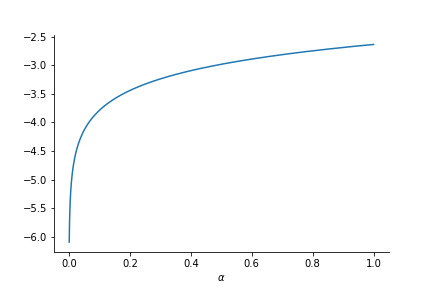
\includegraphics{uStarAlpha}
\caption{Optimal utility as a function of $\alpha$}
\end{figure}


\section{Allocation of time and the values of travel time and reliability with random travel time }

\subsection{Optimal time allocation with random trip duration}

Suppose travel time $T$ is a random variable with a distribution bounded between $0$ and $Q$ \textit{such that the time constraint
is never exceeded}. We parametrise travel time in a convenient form $T=\mu+\sigma X$, where $\mu$ is its mean, $\sigma$ its standard
deviation and $X$ is a standardised random variable with zero mean and unit variance and a probability density function $f\left(X\right)$. The bound on the distribution of $T$ implies that the distribution of $X$ is also bounded between $-\frac{\mu}{\sigma}$ and $\frac{Q-\mu}{\sigma}$. 

Utility is stochastic since it depends on the unknown travel time, $T$. Thus, the exact outcome for a given allocation of time $\left(t_{h},t_{w}\right)$ cannot be determined before the trip. We assume the commuter allocates his/her total time across activities in view of a known travel time distribution. The decision is taken sequentially. Firstly, time at home is optimally allocated between the home-based and mobile activities for any given travel duration and time devoted to the work-based activity. Once travel time is realised upon arrival at work, the commuter optimally allocates the remaining time between the work-based and mobile activities.

We solve the utility maximisation problem by backward induction: Conditional on the information at the time of arrival at work, the commuter determines the optimal time to be allocated to the work-based activity given the realised travel time and the time devoted to the home-based and mobile activities. Then, the optimal time for the home-based activity is determined considering the distribution of travel times.

Upon arrival at the destination, the commuter has $Q-T-t_{d}$ time units to be allocated between the mobile and work-based activities.
As travel time is realised, the commuter faces no uncertainty and his/her problem amounts to:
\begin{gather*}
\max_{t_{w}} \, U_{m}\left(Q - \left(1 - \alpha\right) \left(\mu + \sigma X\right) - t_{h} - t_{w}\right) + U_{w}\left(t_{w}\right)\\
\mbox{s.t. }t_{w}\leq Q-\mu-\sigma X-t_{d}.
\end{gather*}
The constraint indicates that the time that will be allocated to the work-based activity cannot exceed the total available time at the
destination. The Lagrangian of the maximisation problem will be%
\begin{equation*}
U_{m}\left(Q-\left(1-\alpha\right)\left(\mu+\sigma X\right)-t_{h}-t_{w}\right)+U_{w}\left(t_{w}\right)+\eta\left(Q-\mu-\sigma X-t_{d}-t_{w}\right),
\end{equation*}
with first-order conditions for an optimum being%
\begin{subequations}
\label{eq:tw_stage}
\begin{align}
U_{w}^{\prime}\left(t_{w}\right)-U_{m}^{\prime}\left(Q-\left(1-\alpha\right)\left(\mu+\sigma X\right)-t_{h}-t_{w}\right)-\eta & =0
\label{eq:stage2_wrt_tw}\\
\eta\left(Q-\mu-\sigma X-t_{d}-t_{w}\right) & =0\label{eq:stage2_compl}\\
\eta,t_{w} & \geq 0
\label{eq:stage2_nonnegative}
\end{align}
\end{subequations}

If the constraint is non-binding, then the optimal time allocated to the work-based activity, $\hat{t}_{w}$, will be that which equates the marginal utility of time in the work-based and mobile activities:
\begin{equation*}
\hat{t}_{w}=\left\{ t_{w}:U_{w}^{\prime}\left(t_{w}\right)-U_{m}^{\prime}\left(Q-\left(1-\alpha\right)\left(\mu+\sigma X\right)-t_{h}-t_{w}\right)=0\right\} .
\end{equation*}
If however the constraint is binding, then all the time at the destination will be used to carry out the work-based activity, hence $\hat{t}_{w}=Q-t_{d}-\mu-\sigma X$. In this case, the marginal utility of time in the work-based activity will be higher than that in the mobile activity. This is so since, if this was not the case, then the commuter will be better off allocating some of the time at the destination to the mobile activity. If there exists a pair $\left(\hat{t}_{w},\hat{\eta}\right)$ satisfying the first-order conditions in (\ref{eq:tw_stage}), then the optimal utility will be:
\begin{equation*}
V\left(\hat{t}_{w};t_{h}\right)\equiv U_{m}\left(Q-\left(1-\alpha\right)\left(\mu+\sigma X\right)-t_{h}-\hat{t}_{w}\right)+U_{w}\left(\hat{t}_{w}\right)+\hat{\eta}\left(Q-\mu-\sigma X-t_{d}-\hat{t}_{w}\right).
\end{equation*}

Given the optimal allocation of time at work, the commuter will determine the optimal allocation of his/her total time at the origin between the mobile and home-based activities. This decision is made in light of the travel time distribution as the exact travel time is not known before the trip is taken. The commuter chooses the time for the home-based activity in order to maximise expected utility:
\begin{align}
\begin{split}
\max_{t_{h}} \, & E\left[U_{h}\left(t_{h}\right)+V\left(\hat{t}_{w};t_{h}\right)\right]\\
& \mbox{subject to } \, t_{h} \leq t_{d}
\end{split}
\label{eq:firstStageProblem}
\end{align}
where the expectation is over all possible values of the standardised travel time, $X$. The Lagrangian of the utility maximisation problem can be given as: 
\begin{equation*}
E\left[U_{h}\left(t_{h}\right)+U_{m}\left(Q-\left(1-\alpha\right)\left(\mu+\sigma X\right)-t_{h}-\hat{t}_{w}\right)+U_{w}\left(\hat{t}_{w}\right)+\phi\left(t_{h}-t_{d}\right)\right]
\end{equation*}
with first-order conditions
\begin{subequations}\label{eq:th_stage}
\begin{align}
E\left[U_{h}^{\prime}\left(t_{h}\right)-U_{m}^{\prime}\left(Q-\left(1-\alpha\right)\left(\mu+\sigma X\right)-t_{h}-\hat{t}_{w}\right)-\phi\right] & =0
\label{eq:stage1_wrt_th}\\
\phi,t_{h} & \geq 0 
\label{eq:stage1_lambda}\\
\phi\left(t_{d}-t_{h}\right) & =0
\label{eq:stage1_lambdai_const}
\end{align}
\end{subequations}

An optimal allocation exists if there is a quartet $\left(\hat{t}_{h},\hat{t}_{w},\hat{\eta},\hat{\phi}\right)$ satisfying the conditions in (\ref{eq:tw_stage}) and (\ref{eq:th_stage}). The existence and uniqueness of such an optimum is given in the following theorem:
\begin{theorem}
\label{thm:existence_stochastic}Suppose $T<Q$ and that, for $i=\left\{ h,w,m\right\} $, each utility component $U_{i}$ is increasing, strictly concave and twice-continuously differentiable. Then, there exists an optimal time allocation, $\left(\hat{t}_{h},\hat{t}_{w}\right)$, and multipliers $\hat{\eta}$ and $\hat{\phi}$ satisfying (\ref{eq:tw_stage}) and (\ref{eq:th_stage}). This optimum is is unique.
\end{theorem}

\begin{proof}
\textcolor{brown}{The proof for existence and uniqueness at each stage straightforwardly follows the proof of Theorem 1. The main claim to be proved here is the existence and uniqueness of an optimum jointly in the two stages}. We need to show that $V\left(\hat{t}_{w};t_{h}\right)$ is concave in $t_{h}$. Since $U_{h}$ and $V$ are strictly concave in $t_{h}$, the objective function in the choice for an optimal $t_{h}$ is also concave. Thus, it has an optimal allocation, say $\left(\hat{t}_{h},\hat{t}_{w}\right)$.
Now, The following is needed to prove the existence of an optimal allocation $\left(\hat{t}_{h},\hat{t}_{w}\right)$ and multipliers
$\left(\hat{\eta},\hat{\phi}\right)$: (a) $V$ should be concave in $t_{h}$, which is the case for a given $t_{d}$; (b)
\end{proof}

The optimal allocation and departure times can differ depending on the status of the two time constraints. If the commuter has binding
constraints at both ends of the trip, then $\hat{t}_{w}=Q-t_{d}-\mu-\sigma X$ and the mobile activity will be carried out only while travelling, hence $\hat{t}_{m}=\alpha\left(\mu+\sigma X\right)$. In this case, the expected marginal utility of time in the mobile activity will be lower than that in the home-based or work-based activities. In addition, $\hat{t}_{h}=t_{d}$, hence the commuter will depart as soon as he/she spent the last minute of the time allocated to the home-based activity. This is also the case with binding constraint at home irrespective of the status of the constraint at work.

On the other hand, if both the constraints are non-binding, then the marginal expected utility of time will be equalised across the three activities. This is analogous to the case with deterministic travel time. In this case, the optimal departure time can be any moment between $\hat{t}_{h}$ and $Q-\hat{t}_{w}-\mu-\sigma X$.\footnote{Since the exact travel time is unknown before the trip, the optimal departure time may be determined based on a predicted travel time such as the mean, median or other features of the travel time distribution.} This is also the case if the constraint at home is non-binding irrespective of whether the constraint at work is binding. 

If the commuter has binding constraint at work but non-binding constraint at home, i.e., $\eta>0$ and $\phi=0$, then optimality requires that the expected marginal utility of time in the work-based activity be higher than that in the mobile or home-based activities. In this case, the optimal departure time can be any moment between $\hat{t}_{h}$ and $Q-\hat{t}_{w}-\mu-\sigma X$. Conversely, in the case where the constraint at home is binding while that at work is not, the optimal departure time will be $\hat{t}_{h}$ units of time in the home-based activity, and the expected marginal utility of time in the home-based activity will be higher than that in the mobile or work-based activities.

The optimal expected utility: 
\begin{equation*}
W\equiv E\left[U\left(\hat{t}_{h},\hat{t}_{w}\right)\right]=E\left[U_{h}\left(\hat{t}_{h}\right)+U_{m}\left(Q-\left(1-\alpha\right)\left(\mu+\sigma X\right)-\hat{t}_{h}-\hat{t}_{w}\right)+U_{w}\left(\hat{t}_{w}\right)\right],
\end{equation*}
increases with the productivity of in-vehicle time, $\alpha$. Hence, as was the case with deterministic travel time, an improvement in
the productivity of in-vehicle time is welfare improving.

\subsection*{Example}

\subsection{The value of time and reliability with random travel time}

\subsubsection*{The value of travel time}

The value of travel time can be obtained by enveloping the optimal expected utility:
\begin{alignat*}{1}
-\frac{\mathrm{d}W}{\mathrm{d}\mu} & =E\left[U_{w}^{\prime}\left(\hat{t}_{w}\right)-\alpha U_{m}^{\prime}\left(Q-\left(1-\alpha\right)\left(\mu+\sigma X\right)-\hat{t}_{h}-\hat{t}_{w}\right)\right]
\end{alignat*}
The value of travel time is the difference in the expected marginal utility of time in the work-based activity and the mobile activity,
with the latter being weighted by the productivity of in-vehicle time relative to time at work or at home. 

If the constraint at the destination is non-binding and travel time is fully productive, then the value of travel time will be zero. However, if the constraint is binding, then the value travel time will be positive even if travel time is fully productive. This result is similar to the case with deterministic travel time. Note that the value of time is not influenced by the status of the time constraint at the origin.
\textcolor{brown}{Why?}
\begin{prop}
The value of travel time decreases with the productivity of in-vehicle time provided that $\vartheta<1$. 
\end{prop}

\begin{proof}
We want to show that 
\begin{align*}
\frac{\partial\left(-\frac{\mathrm{d}W}{\mathrm{d}\mu}\right)}{\partial\alpha}= & E\left[\frac{\partial\hat{t}_{w}}{\partial\alpha}U_{w}^{\prime\prime}\left(\hat{t}_{w}\right)+\alpha\left(\frac{\partial\hat{t}_{h}}{\partial\alpha}+\frac{\partial\hat{t}_{w}}{\partial\alpha}-\mu-\sigma X\right)U_{m}^{\prime\prime}\left(\hat{t}_{m}\right)-U_{m}^{\prime}\left(\hat{t}_{m}\right)\right]<0
\end{align*}
if $\vartheta<1$. The value of reliability declines with the productivity
of in-vehicle time if $\frac{\partial\hat{t}_{h}}{\partial\alpha}\geq0$,
$\frac{\partial\hat{t}_{w}}{\partial\alpha}\geq0$ and $-\alpha\left(\mu+\sigma X\right)U_{m}^{\prime\prime}\left(\hat{t}_{m}\right)-U_{m}^{\prime}\left(\hat{t}_{m}\right)<0$.
To state the latter in terms of $\vartheta$, define $\xi\equiv-\alpha\left(\mu+\sigma X\right)U_{m}^{\prime\prime}\left(\hat{t}_{m}\right)-U_{m}^{\prime}\left(\hat{t}_{m}\right)$
and $\hat{t}_{m}=\alpha\left(\mu+\sigma X\right)+\epsilon$ where
$\epsilon\geq0$. Thus,
\begin{align*}
\xi & =-\left(\alpha\left(\mu+\sigma X\right)+\epsilon\right)U_{m}^{\prime\prime}\left(\alpha\tau+\epsilon\right)-U_{m}^{\prime}\left(\alpha\left(\mu+\sigma X\right)+\epsilon\right)+\epsilon U_{m}^{\prime\prime}\left(\alpha\left(\mu+\sigma X\right)+\epsilon\right)<0,
\end{align*}
if $\vartheta+\frac{\epsilon U_{m}^{\prime\prime}\left(\alpha\left(\mu+\sigma X\right)+\epsilon\right)}{U_{m}^{\prime}\left(\alpha\left(\mu+\sigma X\right)+\epsilon\right)}<1$,
which holds provided that $\vartheta<1$. Thus, it remains to show
that $\frac{\partial\hat{t}_{h}}{\partial\alpha}\geq0$ and $\frac{\partial\hat{t}_{w}}{\partial\alpha}\geq0$.
To see this, differentiate the first-order conditions in (\ref{eq:tw_stage})
and (\ref{eq:th_stage}) to find that:

\begin{align*}
\frac{\partial\hat{t}_{h}}{\partial\alpha}= & \frac{\frac{\partial\hat{t}_{w}}{\partial\alpha}U_{w}^{\prime\prime}\left(\hat{t}_{w}\right)+\frac{\partial\hat{\phi}}{\partial\alpha}-\frac{\partial\hat{\eta}}{\partial\alpha}}{U_{h}^{\prime\prime}\left(\hat{t}_{h}\right)}\\
\frac{\partial\hat{t}_{w}}{\partial\alpha}= & \frac{\frac{\partial\hat{\eta}}{\partial\alpha}+\left(\mu+\sigma X-\frac{\frac{\partial\hat{\phi}}{\partial\alpha}-\frac{\partial\hat{\eta}}{\partial\alpha}}{U_{h}^{\prime\prime}\left(\hat{t}_{h}\right)}\right)U_{m}^{\prime\prime}\left(\hat{t}_{m}\right)}{U_{w}^{\prime\prime}\left(\hat{t}_{w}\right)+U_{m}^{\prime\prime}\left(\hat{t}_{m}\right)\left(1+\frac{U_{w}^{\prime\prime}\left(\hat{t}_{w}\right)}{U_{h}^{\prime\prime}\left(\hat{t}_{h}\right)}\right)}
\end{align*}
Now, examine what happens to $\frac{\partial\hat{t}_{h}}{\partial\alpha}$
and $\frac{\partial\hat{t}_{w}}{\partial\alpha}$ under the following
cases: 
\begin{casenv}
\item If both constraints are binding, then $\frac{\partial\hat{t}_{w}}{\partial\alpha}=\frac{\partial\hat{t}_{h}}{\partial\alpha}=0$. 
\item If both constraints are non-binding, then $\frac{\partial\hat{\phi}}{\partial\alpha}=\frac{\partial\hat{\eta}}{\partial\alpha}=0$, hence $\frac{\partial\hat{t}_{h}}{\partial\alpha}>0$ and $\frac{\partial\hat{t}_{w}}{\partial\alpha}>0$.
\item If $\hat{\phi}>0$ and $\hat{\eta}=0$, then $\frac{\partial\hat{t}_{h}}{\partial\alpha}=\frac{\partial\hat{\eta}}{\partial\alpha}=0$
and $\frac{\partial\hat{t}_{w}}{\partial\alpha}\geq0$. 
\item If $\hat{\phi}=0$ and $\hat{\eta}>0$, then $\frac{\partial\hat{t}_{w}}{\partial\alpha}=\frac{\partial\hat{\phi}}{\partial\alpha}=0$
and $\frac{\partial\hat{t}_{h}}{\partial\alpha}\geq0$.
\end{casenv}
Therefore, since $\frac{\partial\hat{t}_{h}}{\partial\alpha}\geq0$ and $\frac{\partial\hat{t}_{w}}{\partial\alpha}\geq0$, $\frac{\partial\left(-\frac{\mathrm{d}W}{\mathrm{d}\mu}\right)}{\partial\alpha}<0$ if $\vartheta<1$.
\end{proof}

\subsubsection*{The value of reliability }
\begin{definition}
(\textbf{VOR}) The \textbf{\textit{value of reliability}} refers to the maximum amount a commuter is willing-to-pay for a unit reduction in the standard deviation of travel time. Mathematically, the VOR is $-\frac{\mathrm{d}W}{\mathrm{d}\sigma}$.
\end{definition}
The value of reliability can be derived by differentiating the optimal expected utility with respect to the standard deviation of travel
time $\sigma$: 
\begin{align*}
-\frac{\mathrm{d}W}{\mathrm{d}\sigma} & =E\left[\left(1-\alpha\right)XU_{m}^{\prime}\left(Q-\left(1-\alpha\right)\left(\mu+\sigma X\right)-\hat{t}_{h}-\hat{t}_{w}\right)\right].
\end{align*}
The resulting value indicates the weighted gain in expected utility as the commuter performs the mobile activity at either end of the
trip as opposed to while travelling, where the weight is the standardised travel time. If travel time is as productive as time at home or at work, then there is no gain in undertaking the mobile activity at home or at work. As a result, the value of reliability is zero if travel time is fully productive. Irrespective of the status of the two time constraints, the value of reliability is non-negative irrespective of the status of the time constraints. \textcolor{brown}{One would expect the value of reliability to be higher with a binding constraint at the destination?} 
\begin{prop}
The value of reliability is non-negative and it declines with the productivity of in-vehicle time if $\frac{\partial\hat{t}_{m}}{\partial\alpha}\geq0$. 
\end{prop}

\begin{proof}
To show that the value of reliability is non-negative, let
\begin{equation*}
U_{m}^{\prime}\left(Q-\left(1-\alpha\right)\left(\mu+\sigma X\right)-\hat{t}_{h}-\hat{t}_{w}\right)=\begin{cases}
v_{1} & \mbox{ if X >0}\\
v_{2} & \mbox{ if X\ensuremath{\leq0}}
\end{cases}
\end{equation*}%
where $v_{1}$ and $v_{2}$ are positive constants with $v_{1}\geq v_{2}$ since $\frac{\partial U_{m}^{\prime}\left(Q-\left(1-\alpha\right)\left(\mu+\sigma X\right)-\hat{t}_{h}-\hat{t}_{w}\right)}{\partial X}=-\left(1-\alpha\right)\sigma U_{m}^{\prime\prime}\left(\cdot\right)\geq0$. Using this, the value of reliability can be given as,%
\begin{align*}
-\frac{\mathrm{d}W}{\mathrm{d}\sigma} & =E\left[\left(1-\alpha\right)XU_{m}^{\prime}\left(Q-\left(1-\alpha\right)\left(\mu+\sigma X\right)-\hat{t}_{h}-\hat{t}_{w}\right)\vert X>0\right]\\
 & \qquad+E\left[\left(1-\alpha\right)XU_{m}^{\prime}\left(Q-\left(1-\alpha\right)\left(\mu+\sigma X\right)-\hat{t}_{h}-\hat{t}_{w}\right)\vert X\leq0\right]\\
 & =E\left[\left(1-\alpha\right)v_{1}X\vert X>0\right]+E\left[\left(1-\alpha\right)v_{2}X\vert X\leq0\right]
\end{align*}

Noting that $E\left[X\right]=0$ such that $E\left[X\vert X\leq0\right]=-E\left[X\vert X>0\right]$, we have
\begin{align*}
-\frac{\mathrm{d}W}{\mathrm{d}\sigma} & =\left(1-\alpha\right)v_{1}E\left[X\vert X>0\right]+\left(1-\alpha\right)v_{2}E\left[X\vert X\leq0\right]\\
 & =\left(1-\alpha\right)v_{1}E\left[X\vert X>0\right]-\left(1-\alpha\right)v_{2}E\left[X\vert X>0\right]\\
 & =\left(1-\alpha\right)\left(v_{1}-v_{2}\right)E\left[X\vert X>0\right]\\
 & \geq0
\end{align*}
since $v_{1}\geq v_{2}$ and $E\left[X\vert X>0\right]$. Therefore, the value of reliability is non-negative.

Moreover, we intend to show that
\begin{align*}
\frac{\partial\left(-\frac{dW}{d\sigma}\right)}{\partial\alpha}\text{=} & E\left[X\left(\left(1-\alpha\right)\left(\mu+\sigma X-\frac{\partial\hat{t}_{h}}{\partial\alpha}-\frac{\partial\hat{t}_{w}}{\partial\alpha}\right)U_{m}^{\prime\prime}\left(\hat{t}_{m}\right)-U_{m}^{\prime}\left(\hat{t}_{m}\right)\right)\right]<0
\end{align*}
if $\frac{\partial\hat{t}_{m}}{\partial\alpha}\geq0$.\footnote{Alternatively, the requirement for the claim can be stated as%
\begin{equation*}
\left(\frac{\partial\hat{t}_{h}}{\partial\alpha}+\frac{\partial\hat{t}_{w}}{\partial\alpha}\right)\pi<1
\end{equation*}%
where $\pi=-\frac{U_{m}^{\prime\prime}\left(\hat{t}_{m}\right)}{U_{m}^{\prime}\left(\hat{t}_{m}\right)}$ is the coefficient of absolute risk aversion of $U_{m}$.} Since $\frac{\partial U_{m}^{\prime}\left(\hat{t}_{m}\right)}{\partial X}\geq0$, the above inequality holds if $\mu+\sigma X-\frac{\partial\hat{t}_{h}}{\partial\alpha}-\frac{\partial\hat{t}_{w}}{\partial\alpha}\geq0$, which is the case if $\frac{\partial\hat{t}_{m}}{\partial\alpha}=\mu+\sigma X-\frac{\partial\hat{t}_{h}}{\partial\alpha}-\frac{\partial\hat{t}_{w}}{\partial\alpha}\geq0$.
\end{proof}

An increase in the productivity of in-vehicle time reduces the $\left(1-\alpha\right)$ and hence also the value of reliability, but its effect through $t_{m}$ depends on if and how much the optimal allocation of time changes due to a change in $\alpha$. With binding time constraints at both ends of the trip, $\frac{\partial t_{m}}{\partial\alpha}=\mu+\sigma X>0$ since the time optimally allocated to the home-based and work-based activities will remain unchanged. Thus, the value of reliability declines with the productivity of in-vehicle time irrespective of the value of $\frac{\partial t_{m}}{\partial\alpha}$. However, when one or both constraints are inactive, a change in productivity of in-vehicle time also affects the value of reliability through its effect on the optimal allocation of time. Accordingly, an increase in $\alpha$ increases $t_{h}$ or $t_{w}$ or both. As a result, the value of reliability declines with the productivity of in-vehicle time only if $\frac{\partial\hat{t}_{h}}{\partial\alpha}+\frac{\partial\hat{t}_{w}}{\partial\alpha}\leq\mu+\sigma X$.


\section{Discussion and conclusion}

The model examines the optimal allocation of time among different activities and the valuation of travel time and reliability with self-driving cars. It analyses how the values of travel time and reliability changes with increased productivity of in-vehicle time.

\clearpage{}


Showing the existence of an optimal time allocation follows directly from the proof of Theorem 1 if the optimal expected utility function:

\begin{equation*}
V\left(\hat{t}_{w};t_{h}\right)\equiv U_{m}\left(Q-\left(1-\alpha\right)\left(\mu+\sigma X\right)-t_{h}-\hat{t}_{w}\right)+U_{w}\left(\hat{t}_{w}\right)+\hat{\eta}\left(Q-\mu-\sigma X-t_{d}-\hat{t}_{w}\right).
\end{equation*}%
is concave in $t_{h}$. Since utility is continuous in $t_{h}$, concavity follows if $\frac{\partial}{\partial t_{h}}\left(\frac{\partial V}{\partial t_{h}}\right)$. The first derivative is:
\begin{align*}
\frac{\partial V}{\partial t_{h}}= & U_{m}^{\prime}\left(Q-\left(1-\alpha\right)\left(\mu+\sigma X\right)-t_{h}-\hat{t}_{w}\right)\left(-1-\frac{\hat{t}_{w}}{\partial t_{h}}\right)+U_{w}^{\prime}\left(\hat{t}_{w}\right)\frac{\hat{t}_{w}}{\partial t_{h}}+\hat{\eta}\left(-\frac{t_{d}}{\partial t_{h}}-\frac{\hat{t}_{w}}{\partial t_{h}}\right)\\
= & -U_{m}^{\prime}\left(Q-\left(1-\alpha\right)\left(\mu+\sigma X\right)-t_{h}-\hat{t}_{w}\right)<0
\end{align*}
hence,
\begin{align*}
\frac{\partial}{\partial t_{h}}\left(\frac{\partial V}{\partial t_{h}}\right) & =\frac{\partial}{\partial t_{h}}\left(-U_{m}^{\prime}\left(Q-\left(1-\alpha\right)\left(\mu+\sigma X\right)-t_{h}-\hat{t}_{w}\right)\right)\\
 & =U_{m}^{\prime\prime}\left(Q-\left(1-\alpha\right)\left(\mu+\sigma X\right)-t_{h}-\hat{t}_{w}\right)\left(1+\frac{\partial\hat{t}_{w}}{\partial t_{h}}\right)
\end{align*}
Now, if $\hat{\eta}=0$ then from the first-order condition, we have $U_{w}^{\prime}\left(\hat{t}_{w}\right)=U_{m}^{\prime}\left(Q-\left(1-\alpha\right)\left(\mu+\sigma X\right)-t_{h}-\hat{t}_{w}\right)$ and hence
\begin{equation*}
\frac{\partial\hat{t}_{w}}{\partial t_{h}}=-\frac{U_{m}^{\prime\prime}\left(Q-\left(1-\alpha\right)\left(\mu+\sigma X\right)-t_{h}-\hat{t}_{w}\right)}{U_{w}^{\prime\prime}\left(\hat{t}_{w}\right)+U_{m}^{\prime\prime}\left(Q-\left(1-\alpha\right)\left(\mu+\sigma X\right)-t_{h}-\hat{t}_{w}\right)}>0
\end{equation*}
If $\hat{\eta}>0$ then $t_{d}+t_{w}+T-Q=0$ and hence $\frac{\partial t_{d}}{\partial t_{h}}+\frac{\partial t_{w}}{\partial t_{h}}=0$ if $\frac{\partial t_{d}}{\partial t_{h}}=0$ then $\frac{\partial t_{w}}{\partial t_{h}}=0$. Hence, if $\frac{\partial t_{d}}{\partial t_{h}}$

The conclusion is that $V$is concave in $t_{h}$

\clearpage{}

\bibliographystyle{authordate1}
\bibliography{references}

\end{document}















\clearpage{}
\begin{definition}
Consider defining the following
\end{definition}
\begin{enumerate}
\item Time allocation: A pair $\left(t_{h},t_{w}\right)$ indicating a commuter's
choice of time allocated to the home-based and work-based activities.
\item A time allocation is said to be \textbf{\textit{feasible}} if the
time allocated to the home-based and work-based activities does not
exceed the commuter's time budget less travel time.
\item A continuously differentiable function $f$ is \textbf{\textit{concave}}
if $f^{\prime\prime}<0$.
\item A constraint set is said to be \textbf{\textit{convex}} if a convex
mixture of any two feasible points within the set is also feasible.
\item The \textbf{\textit{value of travel time}} is a commuter's maximum
willing-to-pay for a unit reduction in travel time.
\item The \textbf{\textit{value of reliability}} is the maximum willing-to-pay
for a unit reduction in standard deviation of travel time.
\end{enumerate}
